\section{Comments}\label{section: conclusion}
The hunger game achieves high fidelity (that is, low discrepancy)
for the frequency with which a specified state occurs,
but not for the frequency with which two specified states occur in succession;
the rotor-router game achieves fidelity for the frequency with which
two specified states occur in succession, but not for the frequency 
with which three specified states occur in succession.
One could use a block-encoding trick
(with new states encoding pairs of old states) 
to construct a simulation scheme that
ensures fidelity for the frequency with which
three specified (old) states occur in succession, but at a price:
the resulting rotor-router network will have more rotors,
and hence the quantities that upper-bound discrepancy
in \cite{holroyd2010rotor} will be larger.
Indeed, consider derandomization of a fair coin process.
De Bruijn \cite{debruijn1946} showed that 
for each $k$, there is a cyclic word of length $2^k$
that contains each possible bit-string of length $k$ exactly once;
it follows that if we let $W$ be 
the infinite word associated with this cyclic word,
then for each bit-string $w$ of length $k$,
the unnormalized discrepancy $D(w,n)$,
defined as $n/2^k$ minus the number of apperances of $w$
in the first $n+k-1$ positions of $W$, is bounded.
On the other hand, one cannot find a single infinite word $W$
that accomplishes this task simultaneously for all $k$,
since for example if $w$ is a string containing one or more 1s,
the boundedness of $D(w,n)$
is inconsistent with the occurrence of arbitrarily long strings of 0's.

We propose that a sort of trade-off principle is at work here: 
the more numerical characteristics of a random process
that we attempt to mimic in a deterministic simulation,
the worse our mimicry will be, if our criterion of merit is the rate at which
the simulation's numerical characteristics converge to the limiting values 
of the corresponding numerical characteristics of the random process.
In this context, one sometimes sees the words
``psuedorandom'' and ``quasirandom'',
where a pseudorandom simulation is expected to pass ``all'' tests of randomness
while a quasirandom simulation is expected only to pass certain specified tests.
It is reasonable to expect that the more asymptotic tests of randomness
a quasirandom simulation is required to pass,
the worse the convergence will be.
Indeed, for certain tests of randomness,
the previous assertion is almost a tautology;
for if (say) a random sequence of $0$s and $1$s
had its running average approach 1/2 with discrepancy smaller than $\pm \sqrt{N}$,
that rapidity of convergence would ipso facto
demonstrate negative correlation between the bits,
constituting failure of a correlational test of randomness.

Applying this trade-off principle in the reverse direction,
it seems reasonable to hope that by relaxing our stringency,
and requiring a quasirandom simulation scheme
to pass {\em fewer} tests for randomness,
we enable it to do a {\em better} job
with the tests that it is required to pass;
that is, we make faster convergence possible.
Hence, the delocalized firing mechanism of the hunger game,
by no longer preserving the frequency with which
two specified states occur in succession, may allow
the hunger game to outperform the rotor-router in convergence.

For example, consider the Markov chain with transition matrix
\begin{align*}
    \begin{bmatrix}
        1-q & q \\
        q & 1-q 
    \end{bmatrix}
\end{align*}
with $q$ small, as shown in \cref{fig: conclusion outperform}\,.
\begin{figure}[htbp]
    \centering
    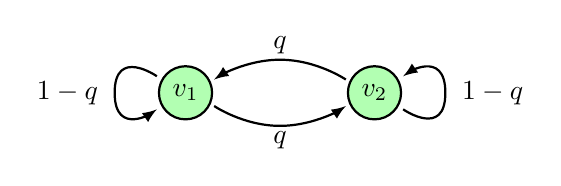
\begin{tikzpicture}[scale=0.6,font=\normalsize,baseline,thick]
        \foreach \x in {1,...,2} {
            \filldraw[color=black,fill=green!30,thick] (4*\x,0) circle (16pt);
            \node at (4*\x,0) {$v_{\x}$};
        }
        % Left arrows
        \foreach \x in {2} {
            \draw [->,>=latex] plot [smooth,tension=1] coordinates {(4*\x-0.866*0.7,0.4*0.7) (4*\x-2,0.7) (4*\x-4+0.866*0.7,0.4*0.7)};
        }
        % Right arrows
        \foreach \x in {1} {
            \draw [->,>=latex] plot [smooth,tension=1] coordinates {(4*\x+0.866*0.7,-0.4*0.7) (4*\x+2,-0.7) (4*\x+4-0.866*0.7,-0.4*0.7)};
        }
        \node at (6,1) {$q$};
        \node at (6,-1) {$q$};
        \draw [->,>=latex] plot [smooth,tension=5] coordinates {(4-0.866*0.7,0.5*0.7) (4-1.5,0) (4-0.866*0.7,-0.5*0.7)};
        \node at (1.5,0) {$1-q$};
        \draw [->,>=latex] plot [smooth,tension=5] coordinates {(8+0.866*0.7,-0.5*0.7) (8+1.5,0) (8+0.866*0.7,0.5*0.7)};
        \node at (10.5,0) {$1-q$};
    \end{tikzpicture}
    \caption{A Markov chain where the hunger game outperforms the rotor-router in convergence}
    \label{fig: conclusion outperform}
\end{figure}
Then under rotor-routing the itinerary of the chip will be
periodic with repeating pattern $1,1,\dots,1,2,2,\dots,2$,
while under the hunger game the itinerary will simply alternate between 1 and 2,
yielding lower discrepancy for the visit-frequencies of the two states.
